\documentclass[../main.tex]{subfiles}
\graphicspath{ {../img/} }


\begin{document}


	\chapter{Our implementation and design}

    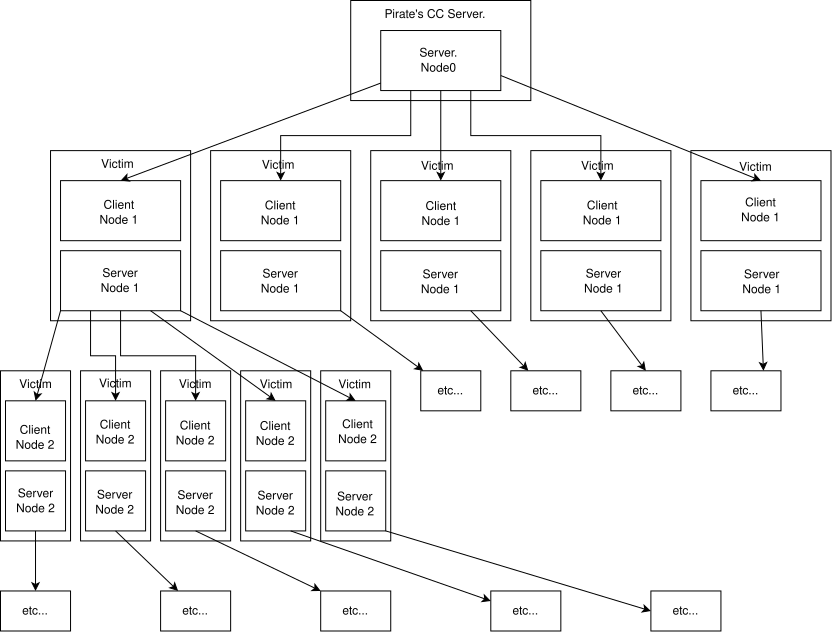
\includegraphics[width=450pt]{botnet.png}

    \vspace{10pt}

    \section{Things necessary for the project we had to either find or makes.}

    Our project had different parts.

    \begin{itemize}

        \item Make a sandboxing environment, to test it, while been sure that it can't escape. 
        We used qemu and unshare to make an environnment that couldn't reach the external network.
        In the end, it wasn't really usefull to make it, because we decided that for the demo, the victims ip should be knowed at launched time, so that we won't see unexpected things in the final demo. 

        \item Find an exploit to use. 
        It had to be a remote code execution, easy to setup, and easy to exploit, because it's not in the purpose of the project to find a new vulnerability, make a exploit or another crazy thing like that.
        We spend hours looking for the perfect exploit, and in the end, we find somebody else project on github, that was doing exactly what we were looking for.
        (https://github.com/opsxcq/
        exploit-CVE-2014-6271)
        Thanks to opsxcq works, we had an easy vulnerability to exploit.
        We choosed shellshock, CVE-2014-6271.
        We find in opsxcq repository, a vulnerable docker image to shellshock CVE-2014-6271, and an easy command to exploit it.
        The other two interested vulnerability that we found in his repos, but that in the end we choosed to not use, was CVE-2016-10033 and CVE-2017-7494.
        There were both unadapted to our needs because of how difficults they would makes us write the exploit.
        We also find Log4J, but in the end decided that we would better to abandon it, and try an easier vulnerability to exploit.

        \item Demonstrate the botnet.
        Like all botnet run things, we had to find a way to prove that the botnet has really taken control of several machine.
        For that, we made one more Vm, that we called vulnerableDOS. We simply run wireshark into, and once the botnet has taken control of the bots, it will make them ping our machine.
        At first, we wanted to make our botnet run an actual DDOS attack on the vulnerableDOS machine, but because it's not in the purpose of the project to make it run a complex attack, our goal is just to prove that we have indeed taken control of the vulnerables machines, we choosed to do only ping.

    \end{itemize}

    Obviously, we also had to make the actual botnet.

    \vspace{10pt}

    \section{design explanations about the botnet.}

    Design and make the botnet was the real challenge. 
    This is what we choosed to do.
    The architecture of our botnet will be a Server, that's gonna do three things.
    first, run the exploit on the victim.
    Second, wait for a response from the victim, to run a Command and Control server (CC), to deliver it's order.
    The first order in the demo will always be to replicate the server on the victim, and the second one to ping the vulnerableDOS vm.
    Third, the server will run a file sharing server (fs), so that everytime the CC server ask the victim to download a file, the file can download it.

    On the CC and the fs server, we implement a TLS connection, using rustls. 
    The certificates used are self signed certificates, and everytime the victim self-replicate the server, it will use the command openssl to generate the certificates.
    We were really lucky that on the vulnerable docker image that we find, there was openssl 1.0f installed. 
    Maybe if the dockerimage was made one or two years earlier, there wouldn't be openssl installed, and we would had to abandon the idea to use encrypted connections.
    We were really lucky.

    The architechture of our botnet will also be composed to a client.
    It's goal will be simply to connect to the server, get it's order, and execute it whatever it is.

    The server will read in a conf folder it's TLS certificates, and the orders file that it will transmit to the victim.
    It will also share some scripts in a www folder, like the list of ips that the next victim have to attack, a config file to easily generate new certificates, the exploit to run in order to run the client on the victim, and an installation script, in order to permit the client to once it has downloaded all the files it needed, to install them correctly, and self replicate the server.

    \vspace{10pt}

    \section{lab setup.}

    To run the demo, we first made a base-vm, with runit-dinit on it, and only basic packages.
    Our goal was to know about everything installed, so that we don't loose time looking for where come a bug from, when it's for a default package.
    Then, we made 1 vm to be the head of our botnet, 2 vulnerable vm, so that when the botnet attack them, they can became bot, and a last one, named vulnerableDOS, with wireshark installed on it.

    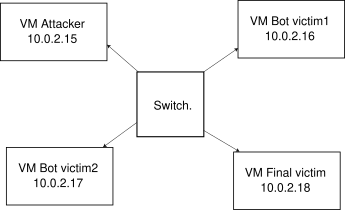
\includegraphics[width=450pt]{lab_env.png}

    Our choice to test the botnet was to make all bots to ping the vulnerableDOS vm.
    That means that our botnet will work if we manage to make bot 1 and 2 to ping vulnerableDOS vm.


    \vspace{10pt}

    \section{Botnet communication.}

    This is the normal functionnement of the botnet.
    Step one. 
    The server find an potential target.
    then, it runs a BASH script, called exploit.sh, which exploit the target.
    That means, exploit the vulnerability, in order to make the victim download and execute the client.
    In our case, the client is installed and ran in `/tmp/botnet/`.

    Step two.
    The client ask the server it's installed order, called order1.
    The server answer, and the client save it in `/tmp/botnet/conf/`.

    Step three.
    The client read the received order, and every time it reach a line begining by `download`, it ask the filesharing server to give it, and put it in `/tmp/botnet/downloaded/`.
    Everytime the client reach a line begining by execute, it's execute the file.

    Normally, the only executed file in the installation phase, it's the script `installation.sh`.
    This script will copy all the downloaded files from `/tmp/botnet/downloaded` to their rightheous folders.
    It will then execute the server.
    The new server will look for other victims, and run again it's CC server and its fs server.

    Finally, once the client had run another server, it will ask for it's attack order from the CC server, which is called order2.
    Typically, an order2 file will ask the client to download and execute a BASH script.
    This BASH script will run the attack.
    In the case of the demo, it will only run `ping 10.0.2.18` to prove that it has made a bot.

    %TODO Put here the comunication draft.

    






\end{document}
